\section{Evaluation}
We now evaluate the performance of Genesis along various dimensions:
 (1) What is the performance of Genesis in synthesizing simple reachability and waypoint policies
  with increasing number of policies and greater sizes of topologies and benchmarking the constraints used by the synthesis algorithm? 
  (2) How quickly can Genesis synthesize isolation policies in datacenter topologies for varying number of policies and percentage of
   datacenter utilization? 
   (3) What is the performance of Genesis for solving link-capacity policies in internet topologies? 
   (4) Identifying the benefits of tactics in terms of reduction of terms in the synthesis algorithm and actual benefits 
   with respect to synthesis without tactics for different isolation workloads in datacenter topologies? 
   (5) What are the potential speedups of using optimistic synthesis in Genesis for varying workloads? 

We model our experimentation on a multi-tenant datacenter setting. We 
define a tenant-group flows as the reachability policies specified by a tenant
for its virtual machines. We evaluate \Name for synthesizing tenant-isolation
workloads for varying sizes of a fat-tree 
topology as a representative datacenter network. For tenant isolation, there are
no isolation policies with packet classes in a tenant-group, but each packet class
has a isolation policy with all other tenant-group packet classes. This setup ensures
that flows of a tenant can share links, but flows of two different tenants cannot share
any link. 
For empirical purposes, 
we perform random allocation
\footnote{Smarter placement of tenants could speed-up synthesis as tenant endpoints would
	be located closer to each other. The placement algorithm can be used to develop specialised tactics.}
 of a tenant's virtual machines to edge switches'
so that the tenant-group flows have random endpoints spread across the datacenter. All 
experiments were conducted using a Cloudlab machine with 32-core Intel-Xeon 2.40GHz CPU and 128Gb of RAM. 
\subsection{Isolation Workloads}
Figure XXX shows the synthesis time (we cap the maximum time at 5000s) for different number of packet classes with varying tenant-group sizes in 80 node fat-tree topology (pod size = 8) without tactics. For example, the total packet classes is 50, and group size is 5 means there are $50/5 = 10$ tenants, and each tenant flow in the group is isolated with all other tenant flows. For a fixed group size, we can observe that as number of packet classes increases, the synthesis time increases expotentially, as expected. As we decrease group size, we can observe that synthesis time increases greatly for the same number of policies, as the number of tenants increases, consequently the problem is more constrainted due to increased number of isolation policies. Group size = 1 denotes the extreme case where all flows are isolated to one other. 

Figure XXY shows the average synthesis time per flow for isolation workloads on increasing fat-tree topology sizes. For this, we fix the group size to 5 and the {\em datacenter packing} ratio to $0.25$. We use the ratio of number of packet classes to number of edge-aggregate links to model the datacenter packing because, in the case of all-to-all isolation, the maximum number of different sources and destination that can be placed at a edge switch is the number of edge-aggregate links at the switch, and thus we cannot have more than $32*4$ tenants in a 80-node topology. As the data packing ratio increases, the synthesis time grows expotentially, and thus, keeping the ratio constant across topologies preserves the relative difficultly of the problem. We are able to synthesize 12 tenants with tenant-group size 5 in a 125-node topology in 124 seconds. We can also observe that average time per flow increases expotential with increasing topology, thus the synthesis problem is expotential with number of nodes as well. 

\subsection{Tactic Reductions}
We can observe that synthesis times for isolation workloads for normal synthesis are not very promising.

%\begin{figure}
%	
%\end{figure}
\begin{figure}
	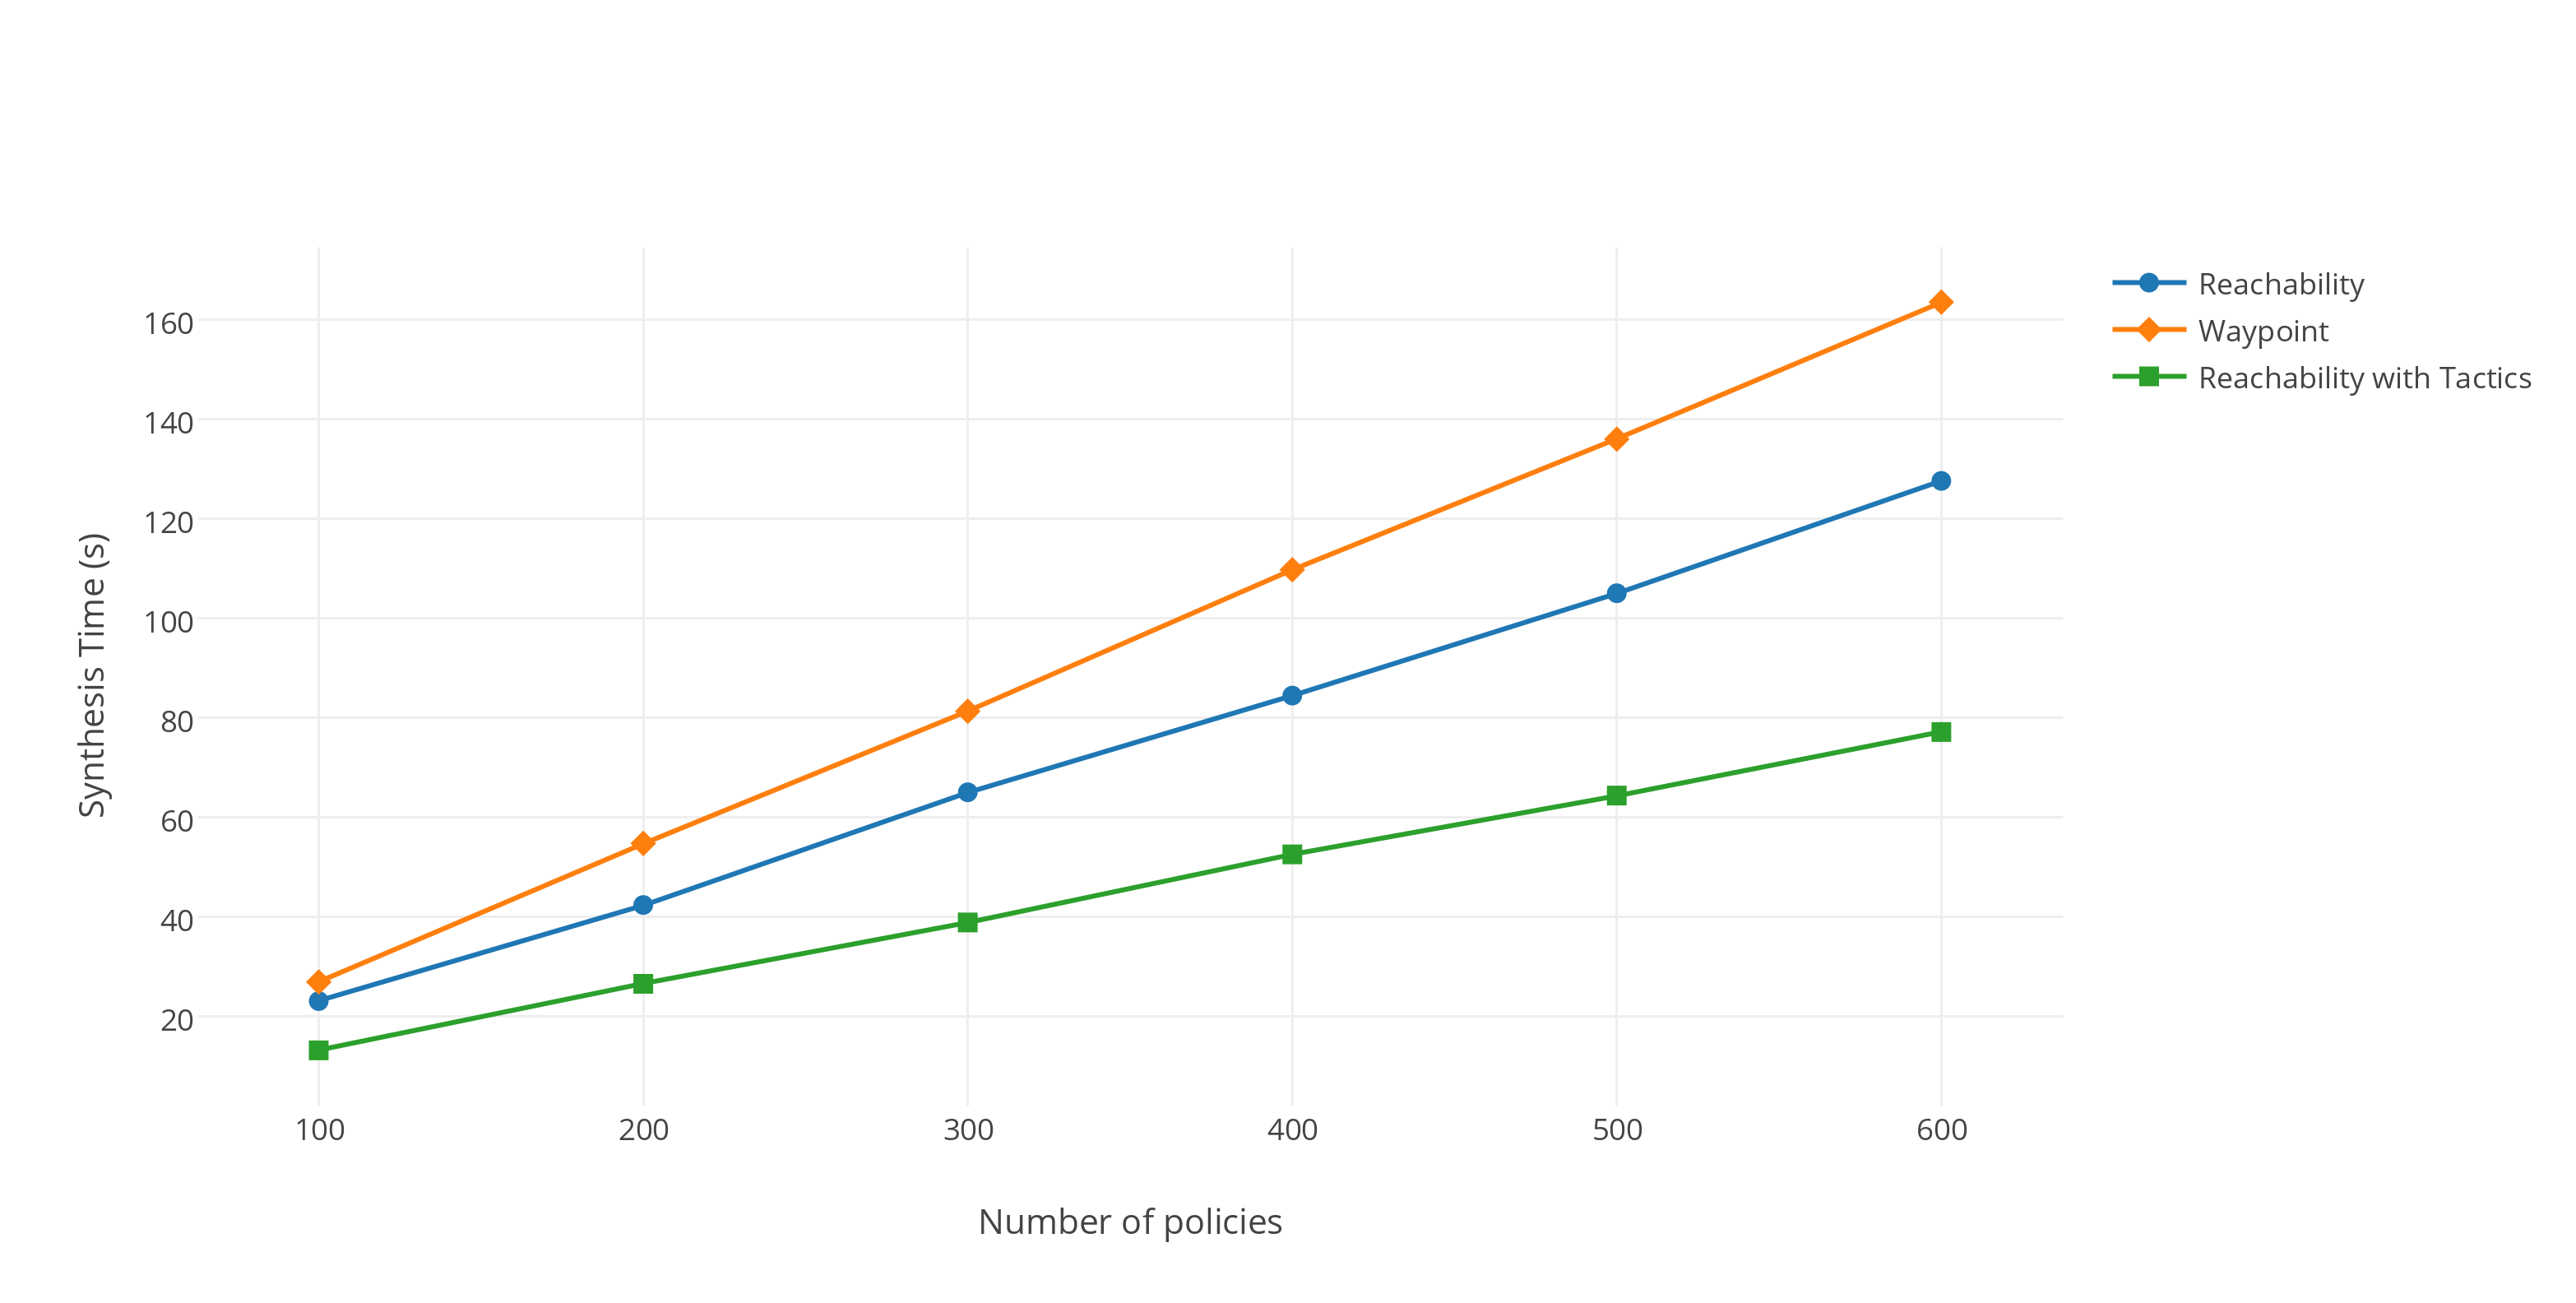
\includegraphics[width=\columnwidth]{figures/reach-way-tactic.png}
	\caption{Graph used to compare time taken for reach v/s waypoint policies in a 45-node fat-tree topology and emphasise due to the generality of the approach we cannot solve reachability using classic algorithms. We therefore need a more heavyweight approach that is slowish. The tactic plot is to show improvements of solving reach using a tactic}
	\label{fig:reach-way-tactic}
\end{figure}
\begin{figure}
	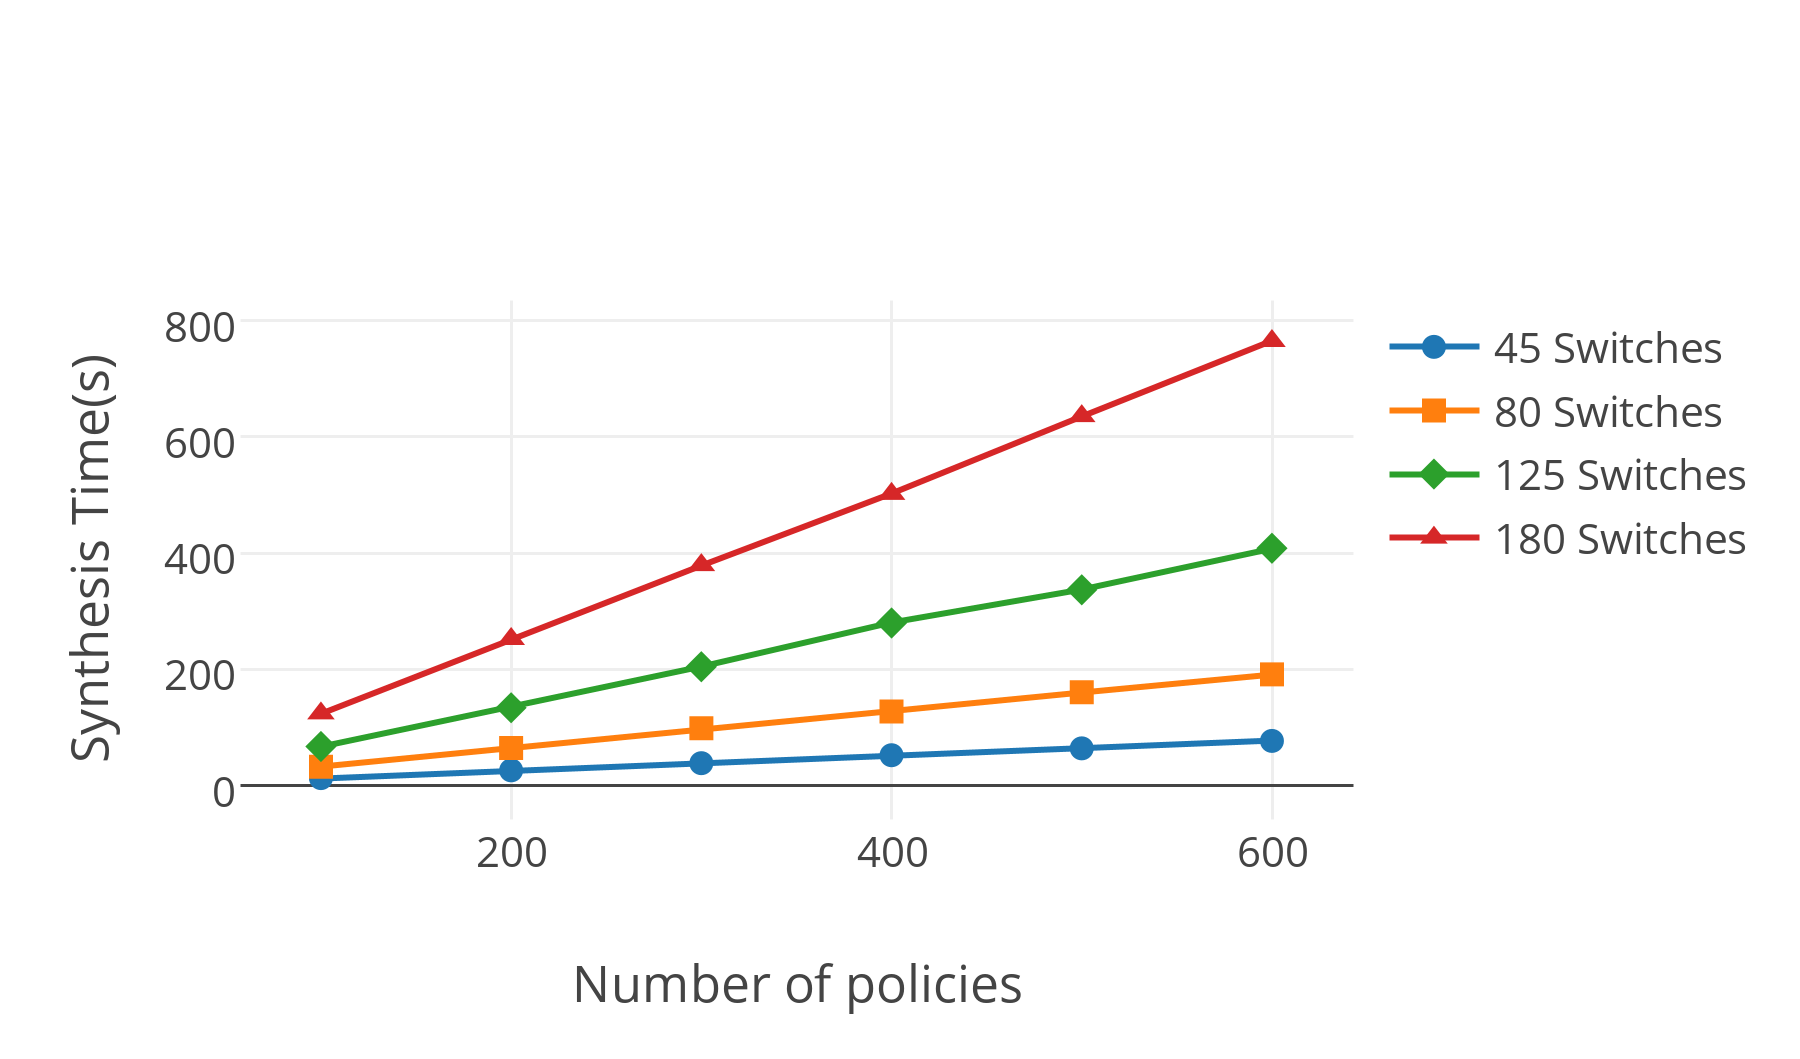
\includegraphics[width=\columnwidth]{figures/reach-topo.png}
	\caption{Graph used to compare time taken for reachability policies for varying topology sizes}
	\label{fig:reach-topo}
\end{figure}


\begin{figure}
	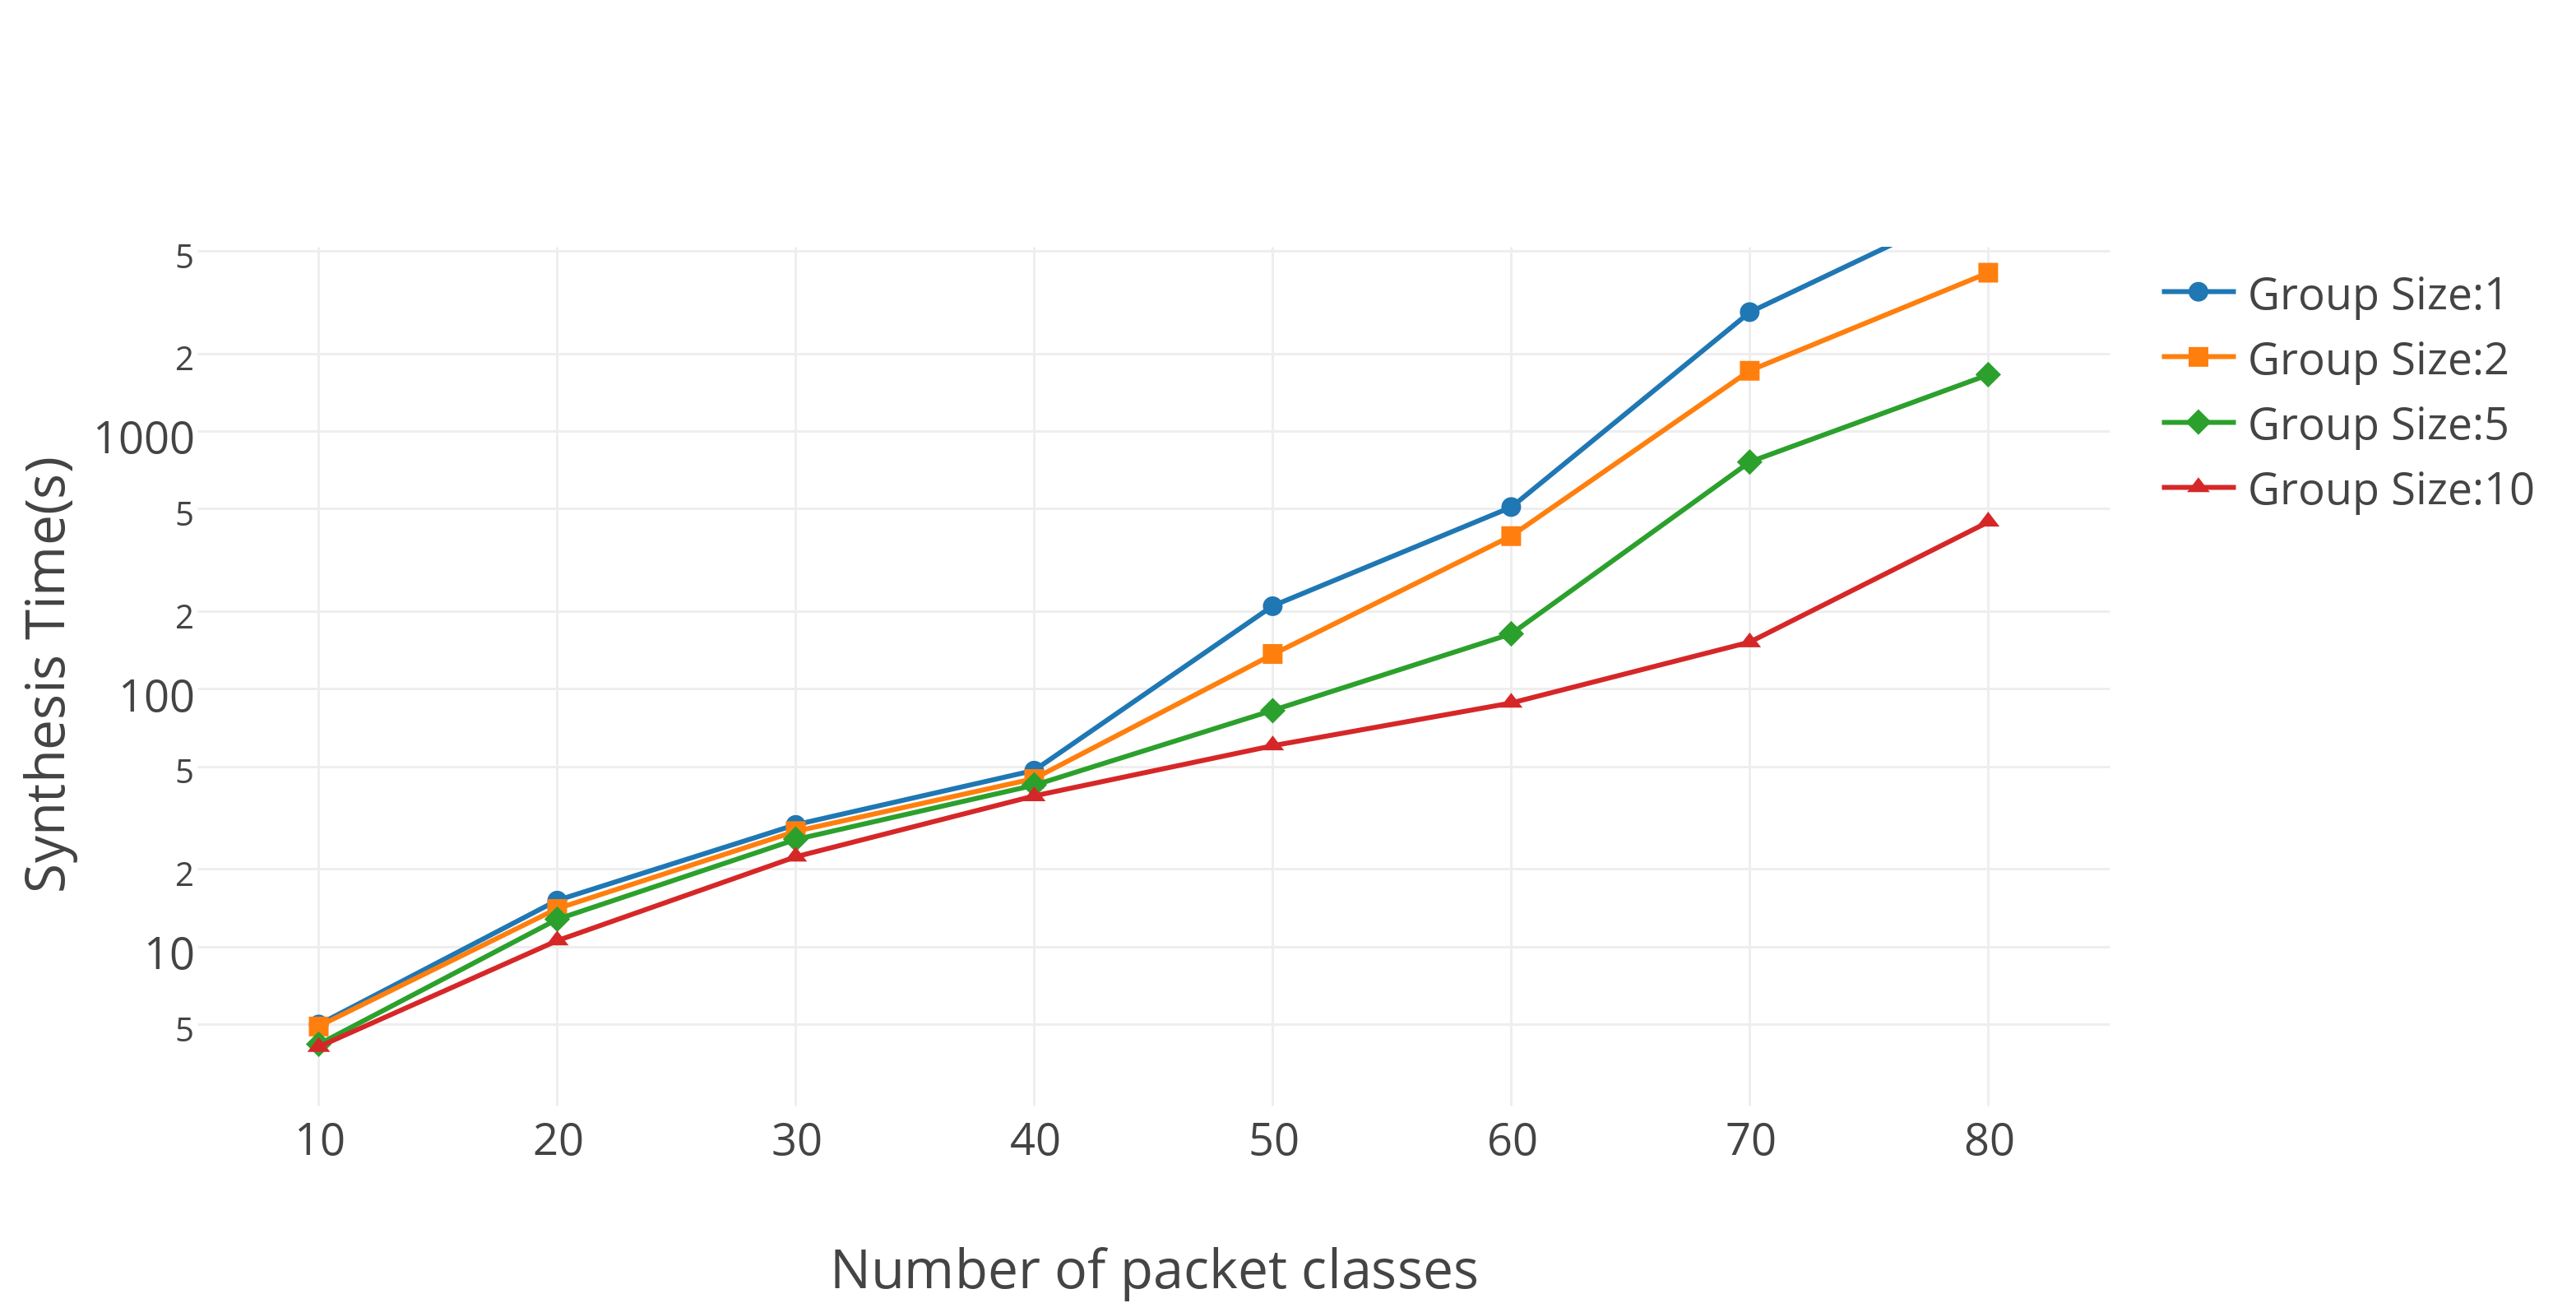
\includegraphics[width=\columnwidth]{figures/performance-isolation-groups-log-scale.png}
	\caption{Graph used to compare time taken for solving isolation policies for varying workloads in a 80 node fat-tree topology}
	\label{fig:isolation}
\end{figure}

\subsection{Tactic Reductions}
\begin{figure*}
	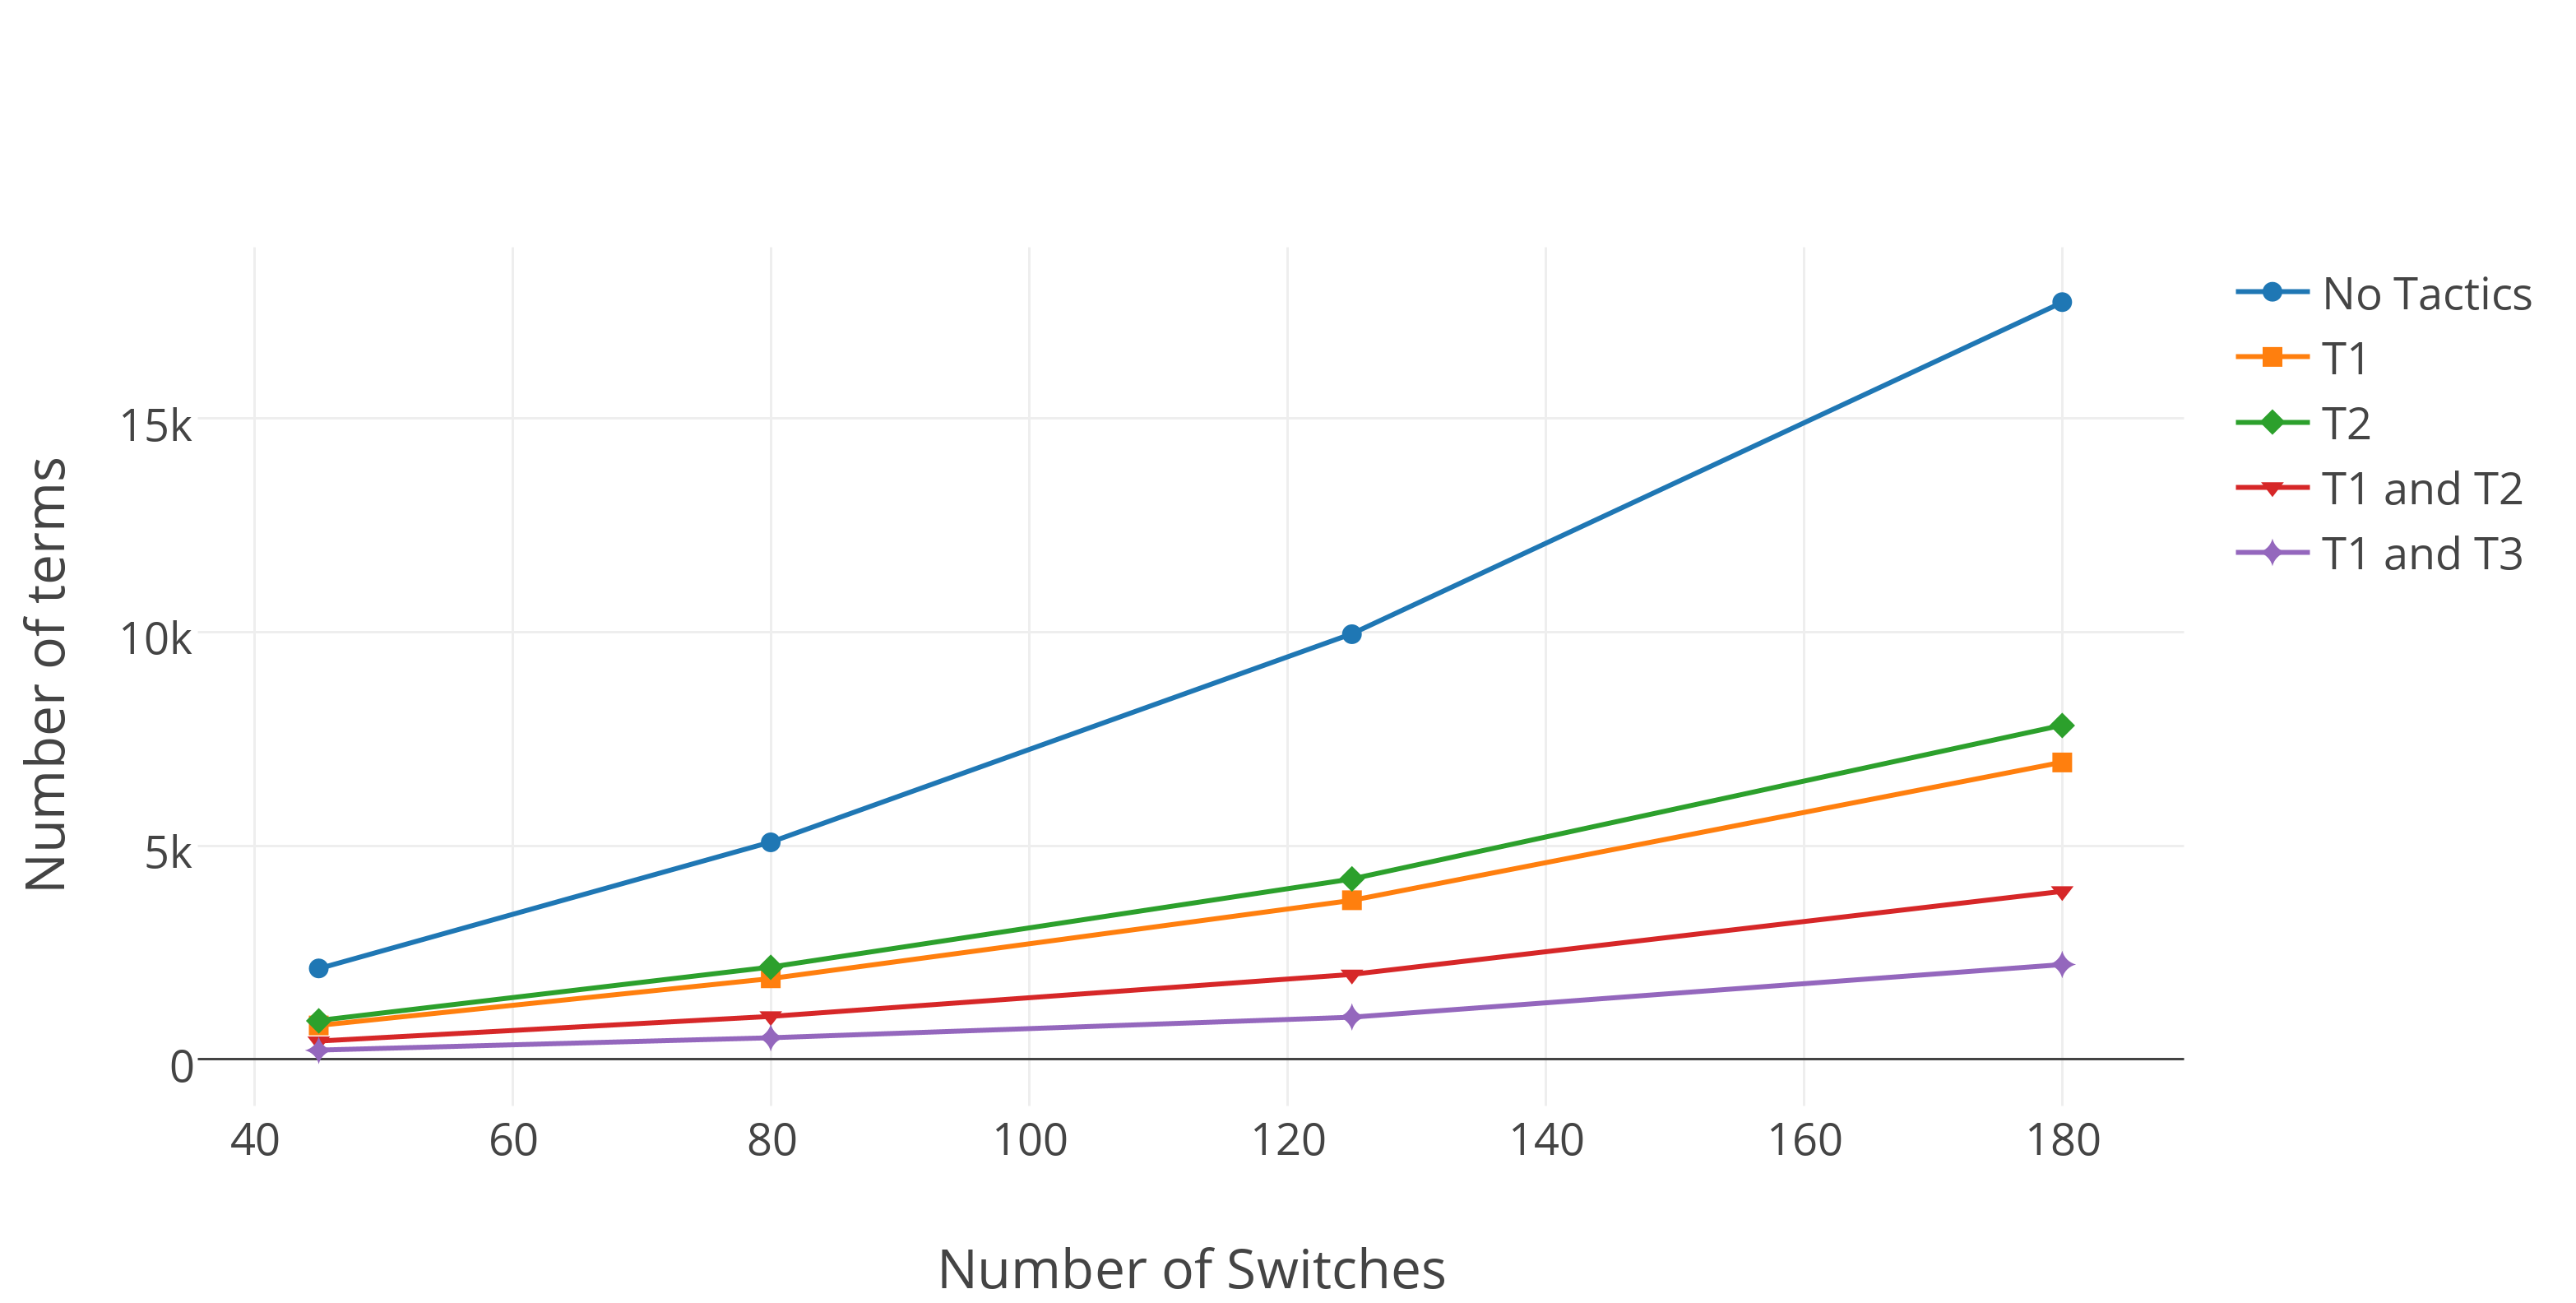
\includegraphics[height=7.5cm]{figures/tactic-reduction.png}
	\caption{Graph used to show the reduction of terms using different tactics w.r.t the total number of terms}
	\label{fig:tactic-reduction}
\end{figure*}

\begin{figure}
	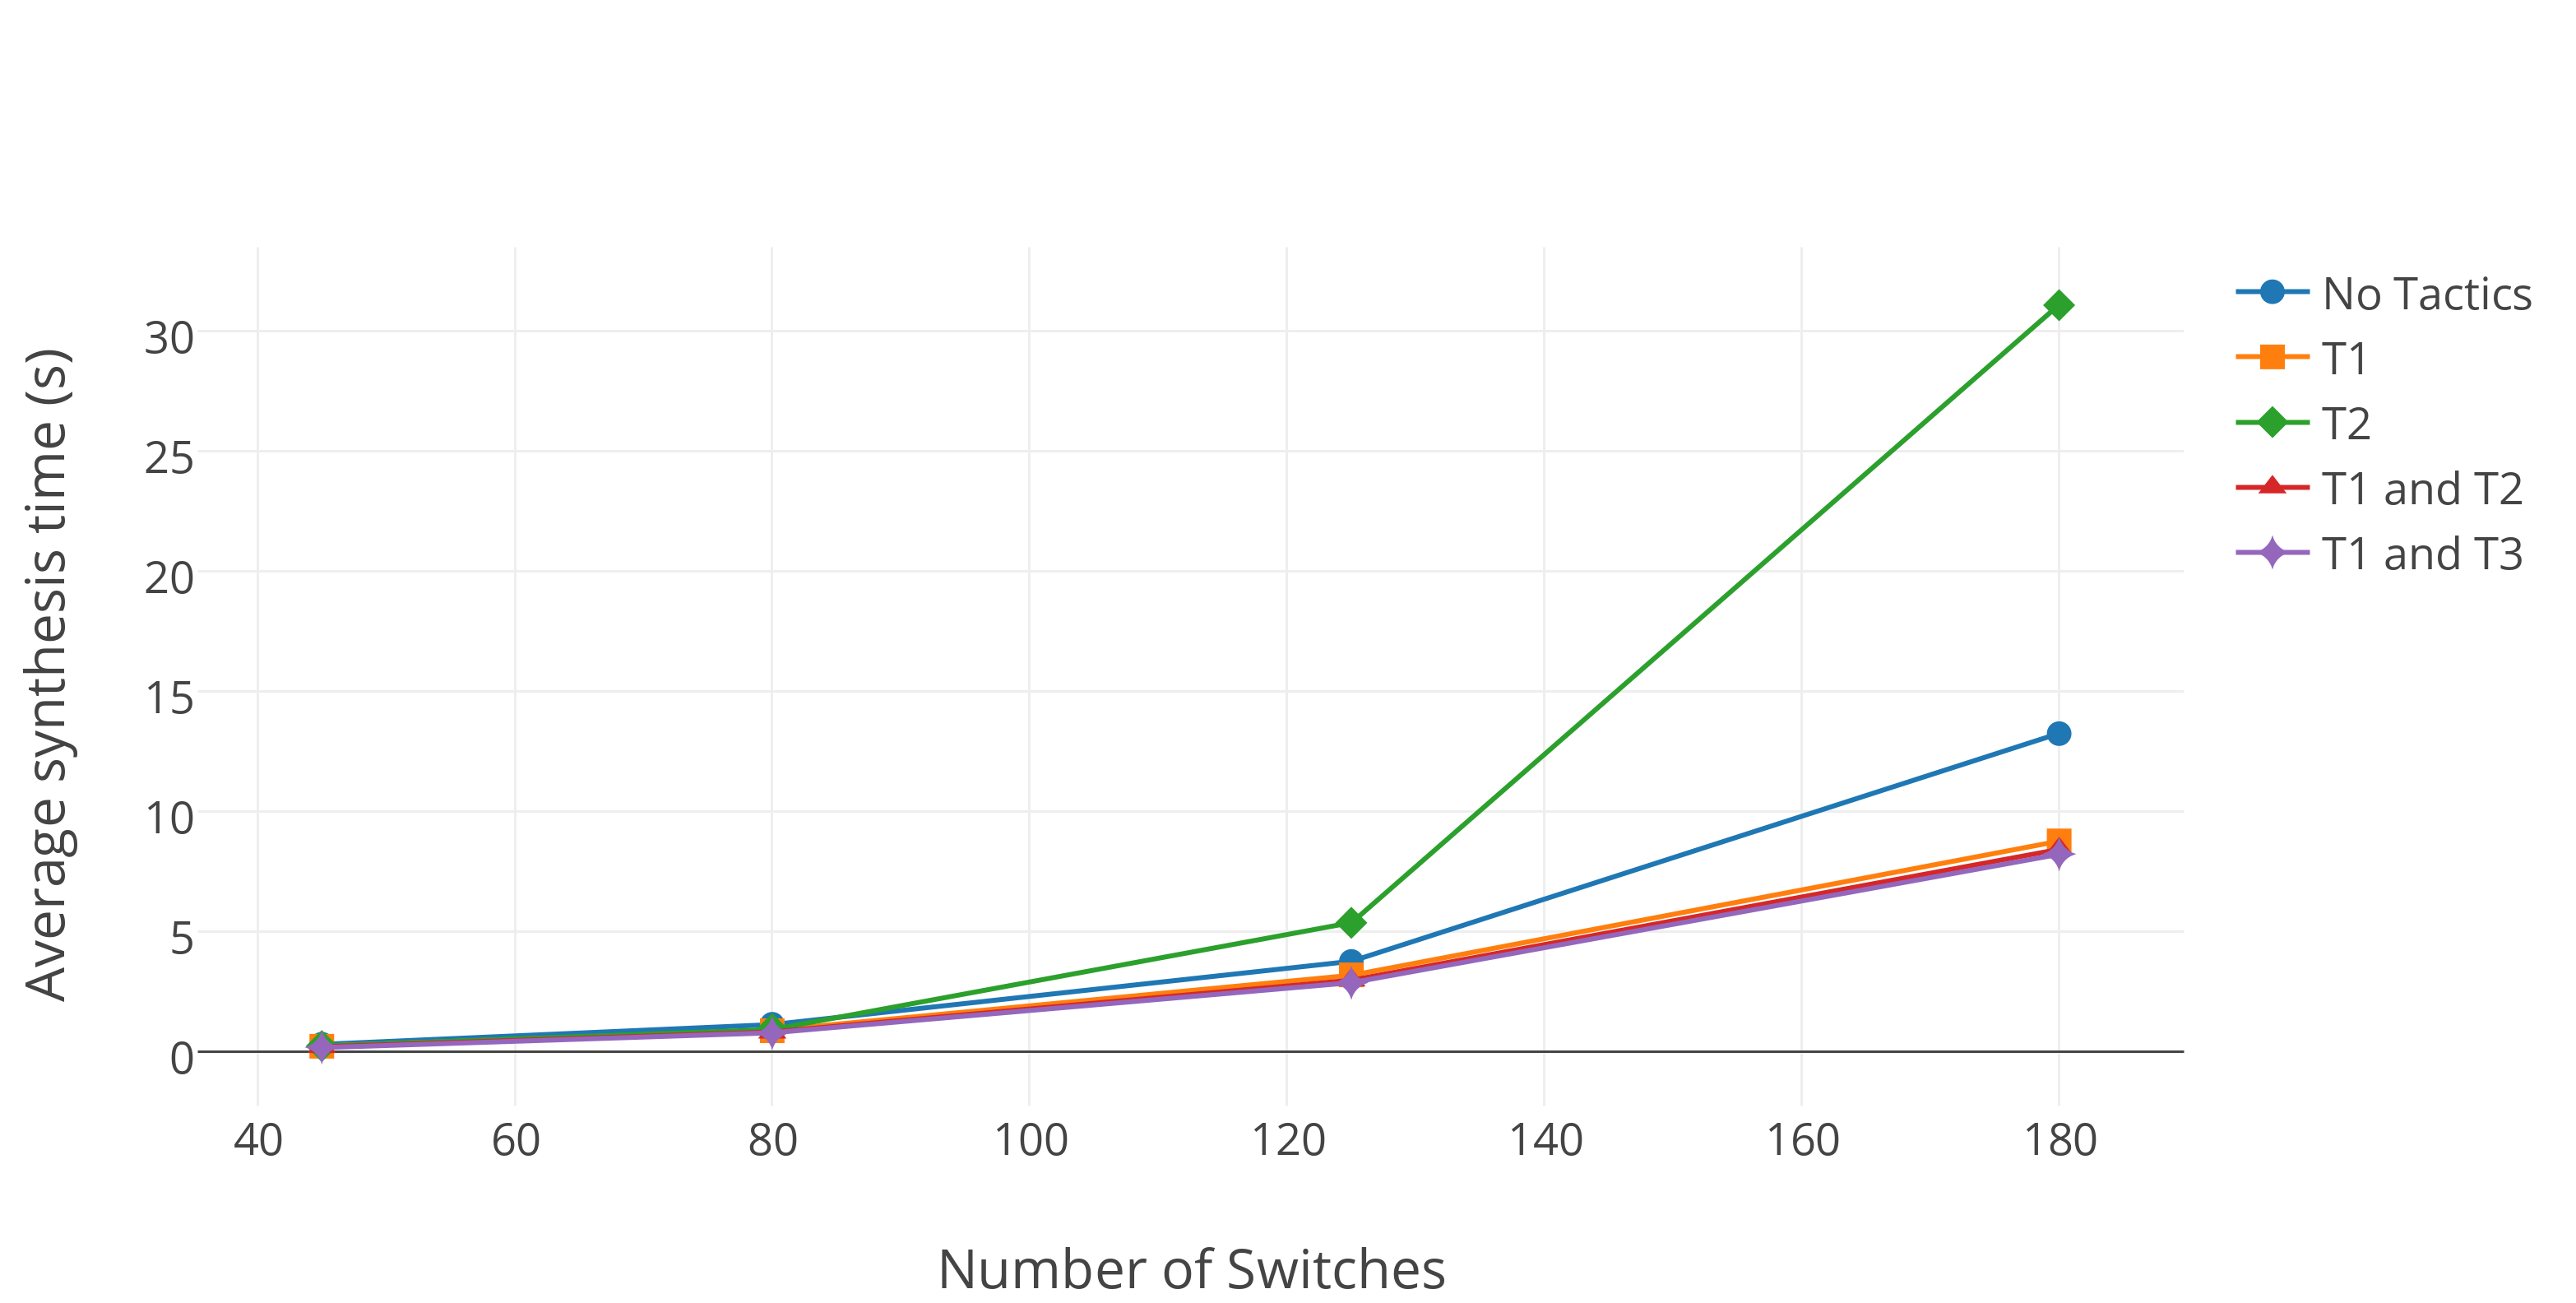
\includegraphics[width=\columnwidth]{figures/isolation-tactics.png}
	\caption{Graph used to application of tactics for a isolation workload (percentage isolation w.r.t topology 25\%) and different topology sizes. An interesting observation in the graph is that tactics need not always help in reduction of constraints (One of the tactics, not  a very natural one) leads to more time to synthesis without tactics.}
	\label{fig:isolation-tactics}
\end{figure}

\subsection{Optimistic Synthesis}
\begin{figure*}
	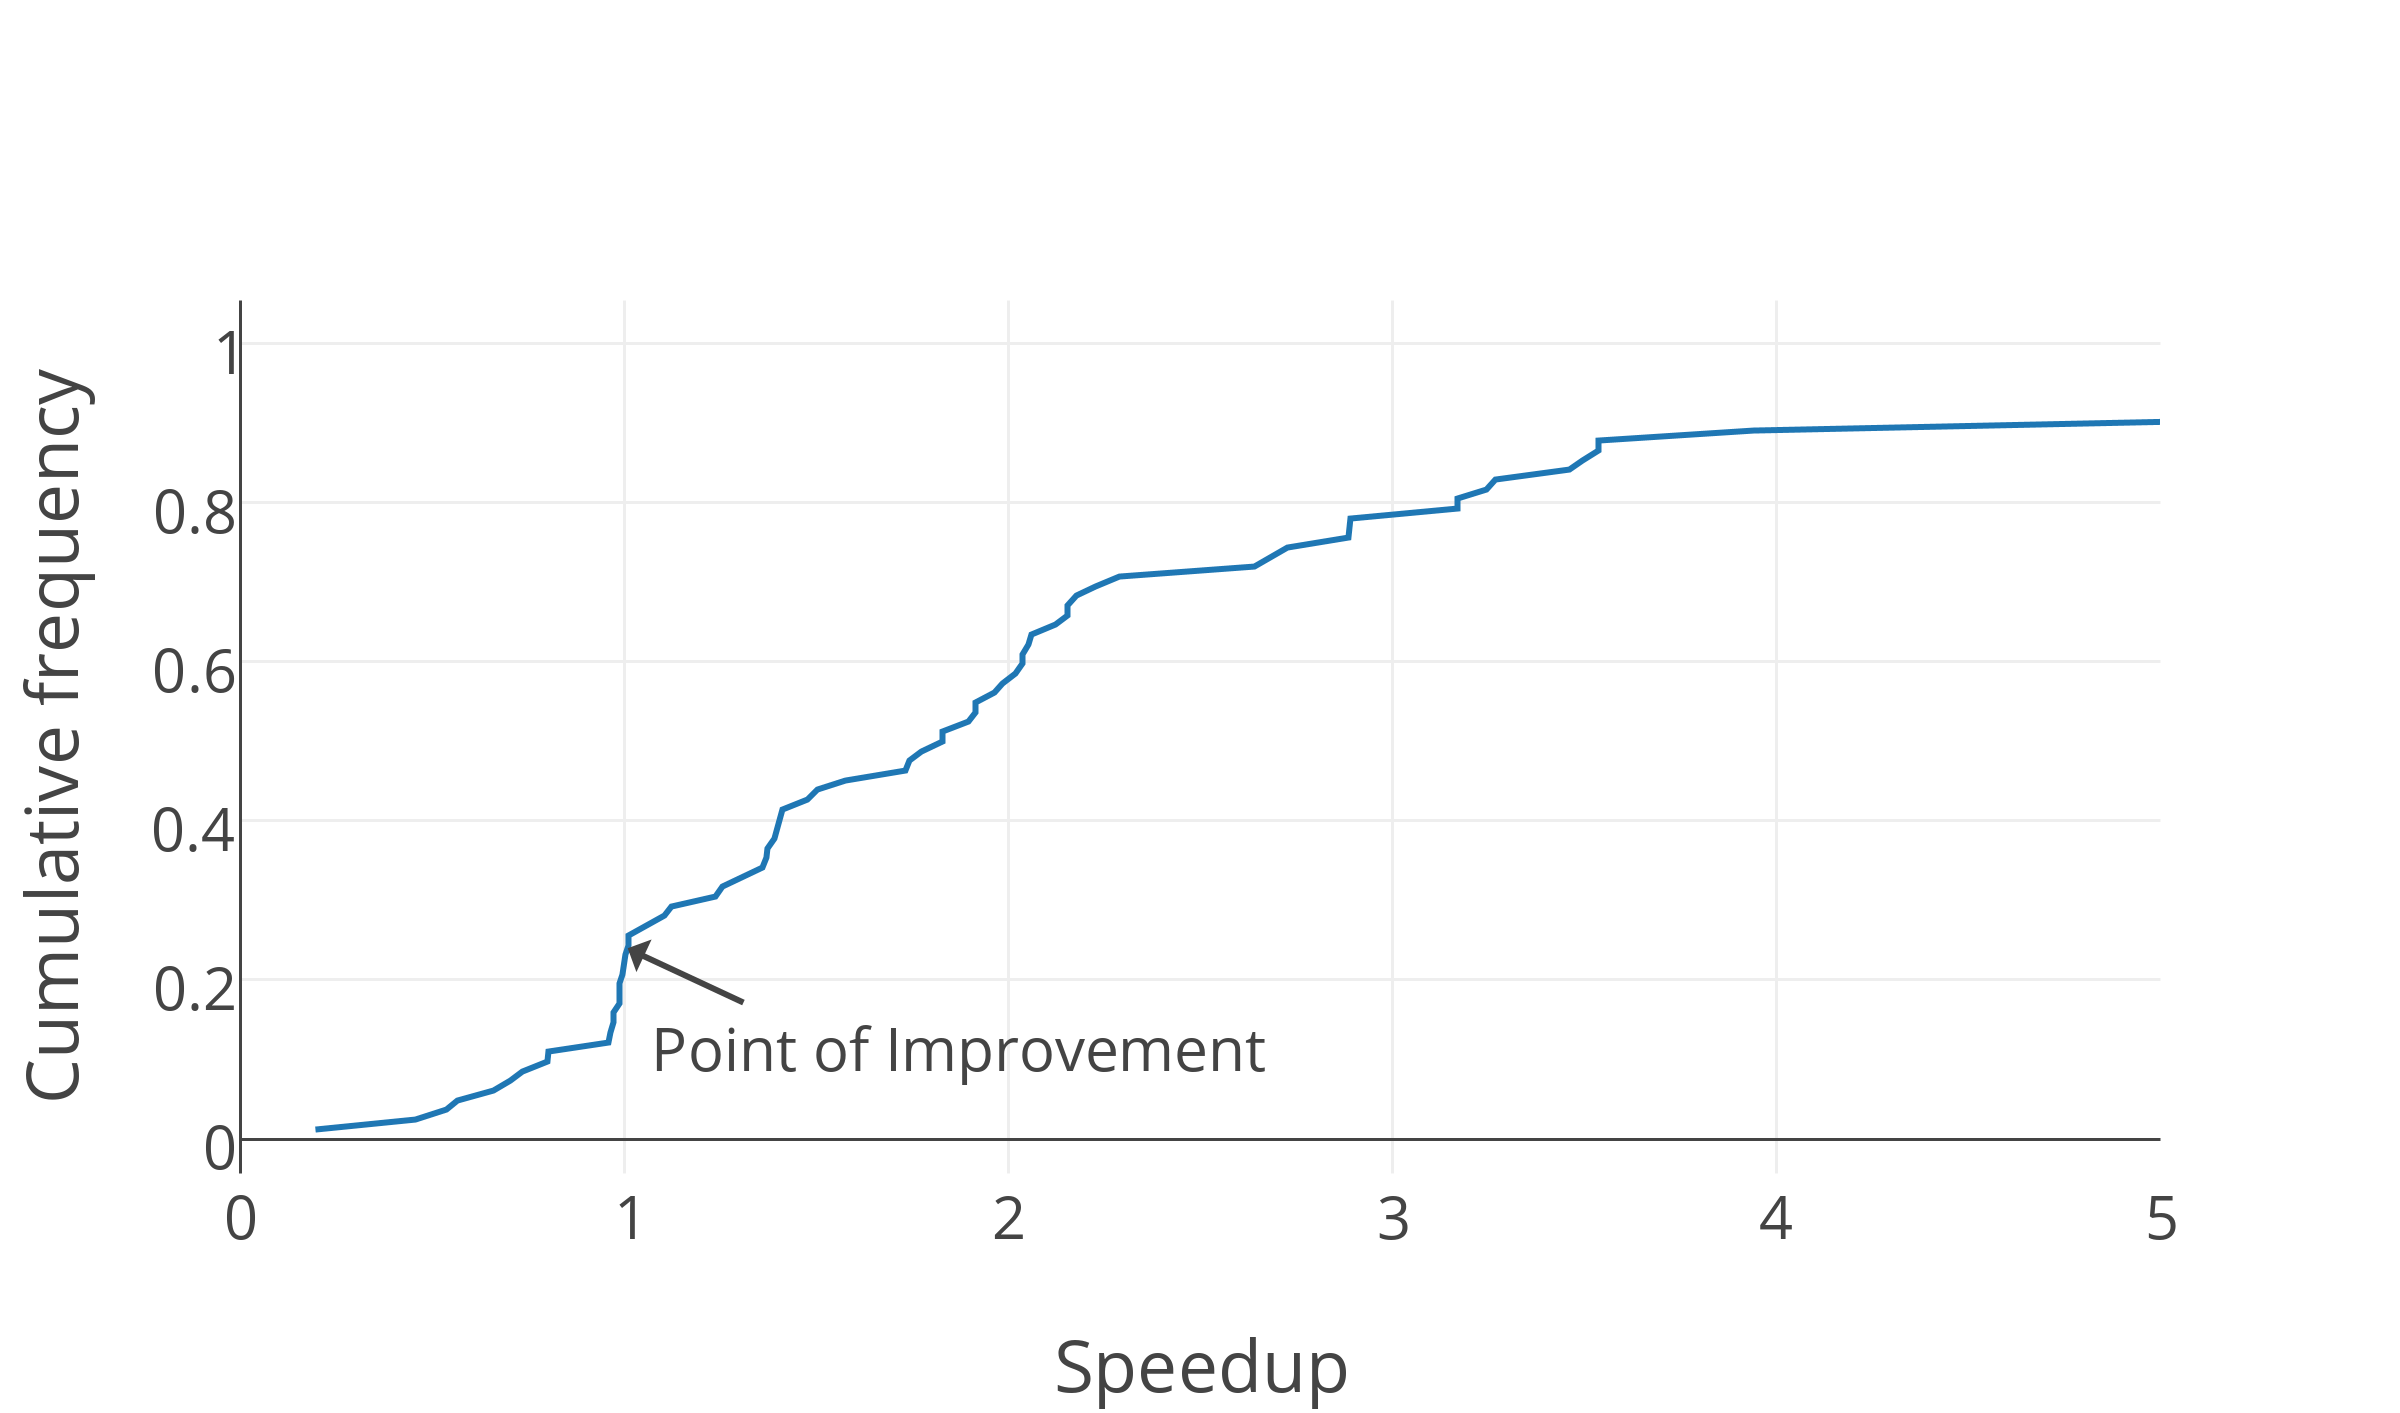
\includegraphics[height=7.5cm]{figures/opt-cdf.png}
	\caption{Graph used to plot the cummulative frequency for speedup achieved by optimistic synthesis (Speedup = optimistic/normal)}
	\label{fig:opt-cdf}
\end{figure*}

\subsection{Incremental Synthesis}
\begin{figure*}
	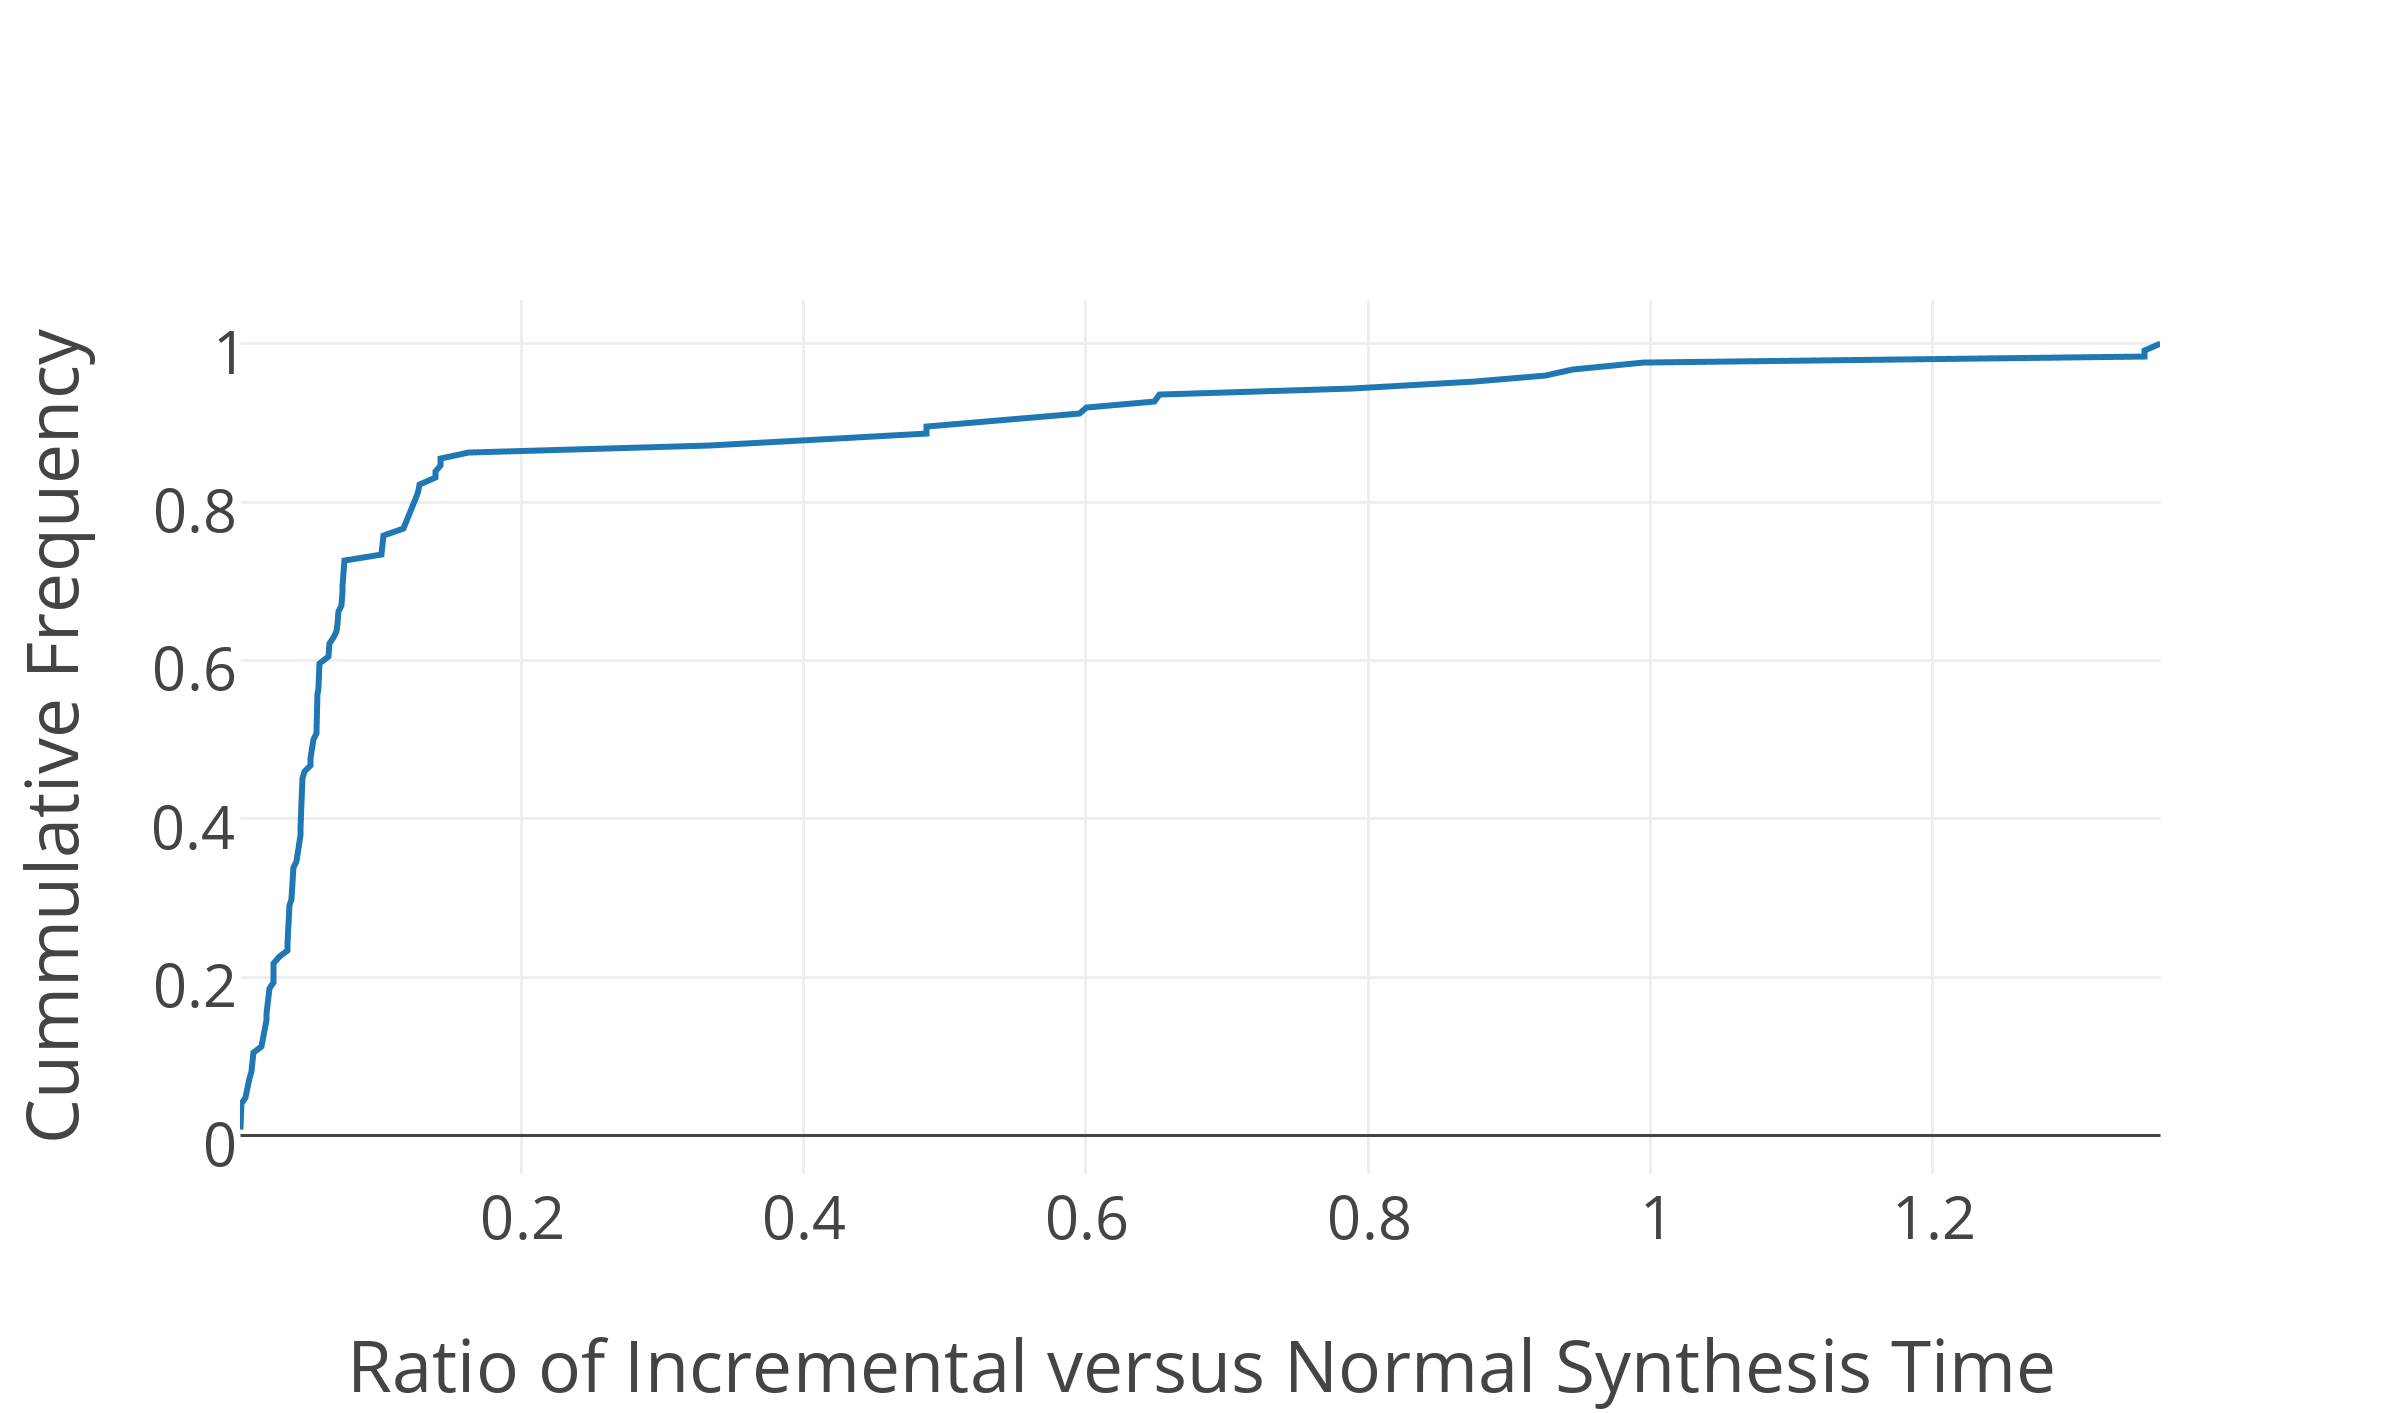
\includegraphics[height=7.5cm]{figures/incremental-cdf.png}
	\caption{Graph used to plot the cummulative frequency for ratio of incremental synthesis/one-shot synthesis.}
	\label{fig:incremental-cdf}
\end{figure*}


%\caption{Synthesis Time for varying number of reachability (with and without tactics) and waypoints policies for a 45 node fat-tree topology}


